%\input{preamble}
%
%\title{\textsc{Probability Theory and Random Processes (MA225)}}
%\subtitle{\textsc{Lecture Slides}\\ Lecture 22 (September 30, 2019) }
%\author{}
%\date{}


\documentclass[10pt]{beamer} %
\usetheme{CambridgeUS}
% \usecolortheme{seahorse}
\usecolortheme{orchid}
% \usepackage[latin1]{inputenc}
\usefonttheme{professionalfonts}
\usepackage{times}
%\usepackage{tikz}
\usepackage{amsmath}
\usepackage{verbatim}
\usepackage{graphicx}
\usepackage{multicol}
%\usetikzlibrary{arrows,shapes}
\setlength{\tabcolsep}{20pt}
\renewcommand{\arraystretch}{1.5}

\usepackage{amsmath,amssymb,amsfonts}
\usepackage{hyperref}
\usepackage{textcomp}
\usepackage[english]{babel}
\usepackage{times}
% \usepackage[T1]{fontenc}

\usepackage{xcolor}
\usepackage{color, colortbl}
\usepackage{multirow}

%\usepackage{beamerthemesplit}
%\usetheme{Warsaw}
\setbeamertemplate{footline}[frame number]
%\usefonttheme{structurebold}
%\usefonttheme[onlymath]{serif}
%\usefonttheme{serif}
\usepackage{pgf,pgfarrows,pgfnodes,pgfautomata,pgfheaps,pgfshade}
\usepackage{amsmath,amssymb}
% \usepackage{inputenc}
%\usepackage[latin1]{inputenc}
\usepackage[english]{babel}
\usepackage{times}
\usepackage{hyperref}
\usepackage{colortbl}
\usepackage{helvet}
\usepackage{booktabs}
\usepackage{multirow}

\usepackage{tikz}
\usetikzlibrary{arrows,shapes,trees, positioning}
\usepackage{graphics}
\usepackage{color}

\pgfdeclarelayer{background}
\pgfdeclarelayer{foreground}
\pgfsetlayers{background,main,foreground}


%\usepackage[dvipsnames]{xcolor}
%\graphicspath{{images/}}
%\renewcommand{\baselinestretch}{1.5}
% \usepackage[utf8]{inputenc} % allow utf-8 input
% \usepackage[T1]{fontenc}    % use 8-bit T1 fonts
%\usepackage{listings}
%\usepackage{hyperref}       % hyperlinks
%\usepackage{url}            % simple URL typesetting
%\usepackage{booktabs}       % professional-quality tables
%\usepackage{amsfonts}       % blackboard math symbols
%\usepackage{nicefrac}       % compact symbols for 1/2, etc.
%\usepackage{microtype}      % microtypography
%\usepackage{lipsum}
% \usepackage{fancyhdr}       % header
%\usepackage{graphicx}       % graphics
%\usepackage{caption}
%\usepackage{subcaption}
%\usepackage[dvipsnames]{xcolor}
%\usepackage{cite}
%\usepackage{epsfig}
%\usepackage{textcomp}
%\usepackage{bm}
%
%\usepackage{algorithm}
%\usepackage{algorithmic}
%\usepackage{dsfont}
%\usepackage{appendixnumberbeamer}
%Header
% \pagestyle{fancy}
% \thispagestyle{empty}
% \rhead{ \textit{ }} 
% \setlength{\tabcolsep}{15pt}


\newcommand{\defn}{\textcolor{red}{Def:~}}
%\AtBeginEnvironment{frame}{\setcounter{myc}{0}}
\newcounter{myc}[section]%framenumber]
\newcommand{\expl}{\textcolor{blue}{\stepcounter{myc}Example~\arabic{myc}:~}}
\newcommand{\theo}{\textcolor{brown}{Theorem:~}}
\newcommand{\coro}{\textcolor{brown}{Corollary:~}}
\newcommand{\remark}{\textcolor{brown}{Remark:~}}
\newcommand{\sam}{\mathcal{S}}
\newcommand{\sig}{\mathcal{F}}
\newcommand{\R}{\mathbb{R}}
\newcommand{\bg}{\boldsymbol{g}}
\newcommand{\bX}{\boldsymbol{X}}
\newcommand{\bx}{\boldsymbol{x}}
\newcommand{\bY}{\boldsymbol{Y}}
\newcommand{\by}{\boldsymbol{y}}
\newcommand{\bt}{\boldsymbol{t}}
\newcommand{\bu}{\boldsymbol{u}}
\newcommand{\bmu}{\boldsymbol{\mu}}
\newcommand{\mc}{\{X_n:n\geq0\}}


\title[]{Statistical Inference and Multivariate Analysis (MA324)}
\subtitle{\textsc{Lecture Slides}\\Topic 03\\ Multiple Linear Regression}
\date{Jan-May 2026}


%\AtBeginSection[]
%{
%	\begin{frame}<beamer>
%		\frametitle{Outline}
%		\tableofcontents[currentsection,currentsubsection]
%	\end{frame}
%}

%\title{\textsc{Probability Theory and Random Processes (MA225)}}
%\subtitle{\textsc{Lecture Slides}\\ Lecture 01 }
%\author{}
%\date{}

\graphicspath{{plots/}}


\begin{document}

% ===================================================================== Frame : Title Page
\thispagestyle{empty}
\maketitle

\begin{frame}
   \frametitle{Multiple Linear Regression}
   \begin{itemize}
      \item In general, the response ($y$) may be related to $p$ regressors (input variables/predictors). 
         \vspace{0.25cm}
      \item The model 
         $$y_i = \beta_0 + \beta_1x_{i1} + \ldots + \beta_px_{ip} + \epsilon_i, i = 1,\ldots,n$$
         is called \textbf{multiple linear regression}. A regression model with $p$  regressors. 
         \vspace{0.25cm}
      \item The parameters $\beta_j, j= 0,1,2,\cdots,p$ are called regression coefficients. 
         \vspace{0.25cm}
      \item $\beta_j, j= 0,1,2,\cdots,p$ represents the change in the average
         value of the response for a unit change in $j^{th}$ regressor keeping
         other regressors fixed. 
         \vspace{0.25cm}
   \end{itemize}


\end{frame}


\begin{frame}
   \frametitle{ }
   \begin{itemize}
      \item Data (of sample size $n$): $(y_i, x_{i1}, x_{i2}, \cdots, x_{ip}), i = 1,\ldots,n$
         \vspace{0.25cm}	
      \item Scalar notation becomes cumbersome -- so matrix notation is used
         \vspace{0.25cm}		
      \item Let
         \begin{displaymath}
            y = \left(
               \begin{array}{c}
                  y_1 \\
                  \vdots \\
                  y_n \\
               \end{array}
            \right), \hspace{0.1cm}  %\quad
            X = \left(
               \begin{array}{cccc}
                  1 & x_{11} & \hdots & x_{1p} \\
                  \vdots & \vdots & x_{ij} & \vdots \\
                  1 & x_{n1} & \hdots & x_{np} \\
               \end{array}
            \right), \hspace{0.1cm} %\quad
            \beta = \left(
               \begin{array}{c}
                  \beta_0 \\
                  \vdots \\
                  \beta_p \\
               \end{array}
            \right), \hspace{0.1cm} %\quad
            \epsilon = \left(
               \begin{array}{c}
                  \epsilon_1 \\
                  \vdots \\
                  \epsilon_n \\
               \end{array}
            \right)
         \end{displaymath}
         \bigskip
      \item Then we can write the model in a more compact form:
         $$ y_{n \times 1} = X_{n \times (p+1)} \beta_{(p+1) \times 1} + \epsilon_{n \times 1}$$
      \item $X$ is called the \textbf{\emph{design matrix}}
   \end{itemize}	


\end{frame}

% == == == == == == == == == == == == == == == == == == == == 
% Frame: Error Assumptions
\begin{frame}
   \frametitle{Error Assumptions}
   \begin{itemize}
      \item As before, $\epsilon_i$'s satisfy
         \begin{itemize}
            \item $E(\epsilon_i) = 0$ for $i= 1,\ldots,n$
               \smallskip
            \item $Var(\epsilon_i)=\sigma^2$ for $i= 1,\ldots,n$
               \smallskip
            \item $Cov(\epsilon_i,\, \epsilon_j) = 0$ for all $i\neq j$
         \end{itemize}
         \bigskip
      \item Equivalently, the assumptions can be written as
         \begin{itemize}
            \item $E\left( \boldsymbol{\epsilon} \right) = \boldsymbol{0}$ 
               \smallskip
            \item $Var(\boldsymbol{\epsilon}) = \sigma^2 I_n$
         \end{itemize}
   \end{itemize}

   
\end{frame}


% \begin{frame}
%    \frametitle{Multiple Linear Regression Model}
%
%    \begin{itemize}
%       \item Multiple Linear Regression Model: 	$$y = X\beta + \epsilon$$
%
%       \item $\epsilon$ is a \textbf{random vector} rather than a random variable.
%          \bigskip
%       \item Assumptions: here, $E(\epsilon) = 0$ and $Var(\epsilon) = \sigma^2I$ and all the assumptions stated in simple linear regression. 
%          \bigskip
%       \item Note that $Var$ is an abuse of notation; in the present context it really means the \textbf{``variance-covariance matrix''.}
%    \end{itemize}	
%
% \end{frame}


\begin{frame}
   \frametitle{Estimation of Regression Coefficients: }
   \begin{itemize}
      \item Consider the objective function
         \begin{eqnarray}
             Q\left( \boldsymbol{\beta} \right)
             &=& Q(\beta_0, \beta_1, \cdots, \beta_p) \nonumber \\
             &=& \sum_{i=1}^{n}\Big(y_i - \beta_0 - \beta_1x_{i1} - \ldots -
             \beta_px_{ip} \Big)^2 \nonumber\\
             &=& (y - X\beta)^T(y - X\beta) \nonumber \\
             &=& \left( y^Ty - 2\beta^TX^Ty + \beta^TX^TX\beta \right) \nonumber
         \end{eqnarray}
      \item The LSEs of $\beta_0, \beta_1, \cdots, \beta_p$ are
         $\displaystyle \operatorname*{arg min}_{\boldsymbol{\beta}} Q\left(
         \boldsymbol{\beta} \right)$.
         % \begin{eqnarray}
         %     &&	\operatorname*{argmin}_{\beta_0, \beta_1, \cdots, \beta_p}
         %     Q(\beta_0, \beta_1, \cdots, \beta_p) \nonumber \\
         %     &=& \operatorname*{argmin}_{\beta_0, \beta_1, \cdots, \beta_p}
         %     \sum_{i=1}^{n}\Big(y_i - \beta_0 - \beta_1x_{i1} - \ldots -
         %     \beta_px_{ip} \Big)^2 \nonumber\\
         %     &=& \operatorname*{argmin}_{\beta} \mbox{ } (y - X\beta)^T(y - X\beta) \nonumber \\
         %     &=& \operatorname*{argmin}_{\beta} ( y^Ty - 2\beta^TX^Ty + \beta^TX^TX\beta) \nonumber
         % \end{eqnarray}
      %    \bigskip
      % \item How to differentiate $Q(\beta)$ with respect to $\beta$?
   \end{itemize}	

\end{frame}

\begin{frame}
    \frametitle{Vector Derivative : Linear Function}
    \begin{itemize}
       \item Let $\boldsymbol{x}$ be an $n \times 1$ column vector (the variable).
       \item Let $\boldsymbol{a}$ be a constant $n \times 1$ column vector.
       \item The derivative of a scalar-valued linear function with respect to
          the vector $\boldsymbol{x}$ is
          \[ \frac{\partial}{\partial \boldsymbol{x}} (\boldsymbol{a}^T
       \boldsymbol{x}) = \boldsymbol{a}. \]
    \end{itemize}
\end{frame}

\begin{frame}
    \frametitle{Vector Derivative: Quadratic Function}
    \begin{itemize}
       \item Let $A$ be a constant $n \times n$ matrix.
          \bigskip
       \item The derivative of a quadratic form with respect to the vector
       $\boldsymbol{x}$ is
          \[ \frac{\partial}{\partial \boldsymbol{x}} (\boldsymbol{x}^T A
          \boldsymbol{x}) = \left( A + A^T \right) \boldsymbol{x}. \]
       \item If $A$ is a symmetric matrix, then the above formula simplifies to
          \[ \frac{\partial}{\partial \boldsymbol{x}} \left( \boldsymbol{x}^T A
             \boldsymbol{x} \right) = 2A \boldsymbol{x}. \]
    \end{itemize}
\end{frame}

\begin{frame}
   \frametitle{Estimation of Model Parameters: }
   \begin{itemize}
      \item Differentiating $Q(\beta)$ with respect to $\beta$ and setting the
         derivative to zero gives the following \emph{normal equations}:
         $$X^TX\beta = X^Ty.$$
      \item The above system of linear equations in $\boldsymbol{\beta}$ is
         always consistent.
         \bigskip
      \item If the matrix $X^TX$ is \emph{invertible} (i.e. if $X$ is of
         \emph{full rank}), then the LSE is unique and given by
         $$\hat\beta = (X^TX)^{-1}X^Ty.$$
   \end{itemize}	
\end{frame}


\begin{frame}
   \frametitle{Fitted Value: }
   \begin{itemize}
      \item The fitted value of response corresponding to regression
         $x = (1, x_1, \cdots, x_p)$ is $$\hat{y} = \hat\beta_0 +
         \hat\beta_1x_{1} + \ldots + \hat\beta_px_{p} $$
      \item Then $\hat y = (\hat y_1, \hat y_2, \cdots, \hat y_n)^T = X\hat\beta
         = X(X^TX)^{-1}X^Ty = Hy$, where, $H = X(X^TX)^{-1}X^T$ is called
         \textbf{hat-matrix}. 
         \vspace{0.5cm}
      \item The residuals: 
         $$\boldsymbol{e}= \begin{bmatrix}
            e_1 \\ \vdots \\ e_n
         \end{bmatrix} 
         = \begin{bmatrix}
            y_1 - \hat y_1 \\ \vdots \\ y_n - \hat y_n
         \end{bmatrix} 
         = \boldsymbol{y}- \hat{\boldsymbol{y}}
         = (I - H)\boldsymbol{y}$$
   \end{itemize}	
\end{frame}

\begin{frame}
   \frametitle{Properties of LSE of $\beta$}
   \begin{itemize}
      \item $\hat{\beta}$ is a linear function of $y$
         \vspace{0.5cm}
      \item $\hat \beta$ is unbiased estimator of $\beta$. That is, $E(\hat \beta) = \beta$
         \vspace{0.5cm}
      \item $
         Var \left( \hat \beta \right) = \sigma^2 (X^TX)^{-1}$
         \vspace{0.5cm}
      \item ${\hat \beta}$ is the BLUE of $\beta$. 
   \end{itemize}	
\end{frame}


\begin{frame}
	\frametitle{Estimation of Error Variance ($\sigma^2$)}
	\begin{itemize}
		\item It can be shown that 
		$$E(SS_{Res}) = (n-p-1) \sigma^2$$
		\vspace{0.01cm}
		
		\item Hence, $\hat\sigma^2 = \frac{SS_{Res}}{n-p-1} = MS_{Res}$ is an unbiased estimator of $\sigma^2$. Here $MS_{Res}$ is residual mean square. 
		\vspace{0.25cm}
		
		\item Observed value of $\hat\sigma^2 = \frac{SS_{Res}}{n-p-1}$ is called \emph{\textbf{Residual variance}}. It's \textbf{square root is called \emph{residual standard error}.}
		\bigskip
\item $\frac{(n-p-1) MS_{Res}}{\sigma^2} \sim \chi_{n-p-1}^2$. 
		\vspace{0.25cm}
		
		\item Here, 
		$$SS_{Res} = \sum_{i=1}^{n} e_{i}^{2} = y^{T}y - \hat{\beta_1^T} X^Ty, $$ 
%		where $$SS_{T} = \sum_{i=1}^{n}(y_i - \bar{y})^2.$$
	\end{itemize}
\end{frame}

\begin{frame}
	\frametitle{Hypothesis Testing: Test for Significance of Regression}
	\begin{itemize}
      \item Assumption: $\boldsymbol{\epsilon}\sim N_n(0, \sigma^2 I_n)$.
      \item Want to test the hypothesis if there is a linear
         relationship between the response $y$ and any of the regressors $x_1,
         \cdots, x_n$:
         $$H_0: \beta_1 = \beta_{2} = \cdots = \beta_p = 0 \mbox{ ag. } H_1:
         \beta_j \neq 0 \mbox{ for atleast one } j = 1,\cdots, p $$
		\item The test statistic is 
         $$ F_0 = \frac{SS_{Reg}/p}{\hat\sigma^2} =
         \frac{SS_{Reg}/p}{SS_{Res}/(n-p-1)} \sim F_{p, n-p-1}, \mbox{ under }
         H_0. $$
		\item Reject $H_0$ iff $F_0 >  F_{p, n-p-1; \alpha}$ (at level $\alpha$) 
	\end{itemize}	
\end{frame}

\begin{frame}
	\frametitle{Hypothesis Testing: Significance of regression coefficients}
	\begin{itemize}
		\item Want to test
		$$H_0: \beta_j = 0 \mbox{ ag. } H_1: \beta_j \neq 0 $$
      \smallskip
   \item Note that $$\hat\beta \sim N_p \left( \beta,\, \sigma^2 \left( X^TX
      \right)^{-1} \right) \implies \hat\beta_j \sim N \left( \beta_j,\,
      \sigma^2 C_{jj} \right),$$
		where $C_{jj}$ is the $j$-th diagonal element of $(X^TX)^{-1}$
		\item The test statistic is 
		$$t_0 = \frac{\hat{\beta_j} }{\sqrt{MS_{Res} C_{jj}}} \sim t_{n-p-1} \mbox{ under } H_0$$
		\item Reject $H_0$ iff $|t_0| > t_{n-p-1, \alpha/2}$ (at level $\alpha$) 
	\end{itemize}	
\end{frame}

\begin{frame}
	\frametitle{Test of contribution of a subset of the regressors}
	\begin{itemize}
		\item \begin{eqnarray}
      y &=& X \beta + \epsilon \implies y = (X_1, X_2) \begin{pmatrix} \beta_1
      \\ \beta_2 \end{pmatrix} + \epsilon \nonumber 
		\end{eqnarray}
   \item Want to test:
		$$H_0: {\beta_2} = 0 \mbox{ ag. } H_1: {\beta_2} \neq 0 $$
   \item Based on the full model (${y} =
      {X} {\beta} + {\epsilon}$),
      ${\hat\beta} = (X^TX)^{-1}X^Ty$ and
      $SS_{Reg}({\beta})$ has $p$ degrees of freedom. 
		\vspace{0.2cm}
      \item To find the contribution of ${\beta_2}$, fit the model
         assuming ${\beta_2} = 0$. 
         \vspace{0.2cm}		
      \item The reduced model is ${y} =
         {X_1} {\beta_1} + {\epsilon}$,
         ${\hat\beta_1} = (X_1^TX_1)^{-1}X_1^Ty$ and
         $SS_{Reg}({\beta_1})$ has $ p-r$ degrees of freedom. Where
         $r$ denotes the number of components in ${\beta_2}$
	\end{itemize}	
\end{frame}

\begin{frame}
	\frametitle{Test of contribution of a subset of the regressors}
	\begin{itemize}
      \item $SS_{Reg}({\beta_2} \mid {\beta_1}) =
         SS_{Reg}({\beta}) - SS_{Reg}({\beta_1})$ can be
         used as a measure of contribution of ${\beta_2}$
         \vspace{0.5cm}
      \item Note that if ${\beta_2}$ has significant contribution
         then $SS_{Reg}({\beta_2} \mid {\beta_1})$ is large
         \vspace{0.5cm}		
      \item Therefore, the test statistic is 
         $$ F_0 = \frac{SS_{Reg}({\beta_2} \mid {\beta_1})/r}{\hat\sigma^2} =
         \frac{SS_{Reg}({\beta_2} \mid {\beta_1})/r}{SS_{Res}/(n-p-1)} \sim F_{r, n-p-1}, \mbox{
         under } H_0$$
      \item Reject $H_0$ iff $F_0 >  F_{r, n-p-1; \alpha}$ (at level $\alpha$)
   \end{itemize}	
\end{frame}

% \begin{frame}
%    \frametitle{Testing of general linear hypothesis}
%    \begin{itemize}
%       \item Want to test:
%          $$H_0: T\undertilde{\beta} = 0 \mbox{ ag. } H_1: T\undertilde{\beta} \neq 0, $$
%          where $T$ is a $m\times (p+1)$ matrix of constants. 
%          \vspace{0.1cm}
%       \item Examples: $y = \beta_0 + \beta_1x_{1} + \beta_2x_{2} + \beta_3x_{3} + \epsilon$
%          \vspace{0.1cm}
%          \begin{itemize}
%             \item 	$H_0: \beta_1 = \beta_{3}  \mbox{ ag. } H_1: \beta_1 \neq \beta_{3}$. Take, $T = \begin{bmatrix}
%                   0 & 1 & 0 & -1
%                \end{bmatrix} $. 
%                \vspace{0.2cm}
%             \item 	$H_0: \beta_1 = \beta_{3}, \beta_{2}=0 \mbox{ ag. } H_1: \beta_1 \neq \beta_{3} \mbox{ or } \beta_{2} \neq 0$. Take, 
%                $$T = \begin{bmatrix}
%                   0 & 1 & 0 & -1  \\
%                   0 & 0 & 1 & 0 
%                \end{bmatrix} $$. 
%          \end{itemize}	
%
%       \item The full model (FM) is $\undertilde{y} = \undertilde{X}\undertilde{\beta} + \undertilde{\epsilon}$, $\undertilde{\hat\beta} = (X^TX)^{-1}X^Ty$ and $SS_{Res}(FM)= y^{T}y - \hat{\beta^T} X^Ty$ has $n-p-1$ degrees of freedom. 
%          \vspace{0.1cm}		
%       \item  Now assume that $T$ has $r (\leq m)$ independent rows. Then $T\undertilde{\beta}$ can be solved and $r$ of the $\beta_j$'s in FM can be written in terms of other $(p+1 - r)$ $\beta_j$'s.
%    \end{itemize}	
%
% \end{frame}
%
% \begin{frame}
% 	\frametitle{Testing of general linear hypothesis}
% \begin{itemize}
% 	\item This lead to the reduced model (RM)  $$\undertilde{y} = \undertilde{Z}\undertilde{\gamma} + \undertilde{\epsilon^*},$$ where $Z$ is $n\times \overline{p+1-r}$ matrix. 
% 	$$\undertilde{\hat\gamma} = (Z^TZ)^{-1}Z^Ty, \mbox{ and } SS_{Res}(RM)= y^{T}y - \hat{\gamma^T} Z^Ty $$ 
% 	 has $n-p-1 + r$ degrees of freedom.
% 	 \vspace{0.2cm}
% 	 \item $SS_{Res}(FM) \leq SS_{Res}(RM)$
% 	 	 \vspace{0.2cm}
% 	 \item Consider $SS_{H} = SS_{Res}(RM) - SS_{Res}(FM)$ with d.f $(n-p-1 + r) - (n-p-1) = r$
% 	 	 \vspace{0.2cm}
% 	 	 		\item Therefore, the test statistic is 
% 	 	 $$ F_0 =  \frac{SS_{H}/r}{SS_{Res}(FM)/(n-p-1)} \sim F_{r, n-p-1}, \mbox{ under } H_0. $$
% \vspace{0.5cm}
% \item Reject $H_0$ iff $F_0 >  F_{r, n-p-1; \alpha}$ (at level $\alpha$). 
% \end{itemize}
% \end{frame}

\begin{frame}
   \frametitle{Confidence intervals for $\beta_j$: }
   \begin{itemize}
      \item Confidence Interval of individual regression coefficient $\hat\beta_j$
         \vspace{0.5cm}
      \item Pivot is
         $$ \frac{\hat{\beta_j} - \beta_{j}}{\sqrt{MS_{Res}C_{jj}}} \sim t_{n-p-1}, $$
         where $C_{jj}$ is the diagonal element of $(X^TX)^{-1}$ matrix. 
         \vspace{0.5cm}
      \item A $100(1-\alpha)\%$ CI for $\beta_j$ is 
         $$\Bigg[\hat{\beta_j} \pm t_{n-p-1, \alpha/2} \sqrt{MS_{Res}C_{jj}} \Bigg]. $$
   \end{itemize}	
\end{frame}

\begin{frame}
   \frametitle{Confidence interval for mean response: }
   \begin{itemize}
      \item  Let ${x_0} = \begin{pmatrix}
            1 \\ x_{01} \\ \vdots \\ x_{0p}
         \end{pmatrix}$ be a value of the regressor vector
      \item The mean response at
         ${x_0}$ is ${x_0}^T\beta$ 
         \vspace{0.2cm}		
      % \item Confidence Interval for mean response  $\undertilde{x_0}^T\undertilde{\beta}$
      %    \vspace{0.2cm}
      \item Pivot is
      $ \frac{\hat{y}_0- {x_0}^T{\beta}}{\sqrt{MS_{Res} {x_0}^T
         (X^TX)^{-1} {x_0}} } \sim t_{n-p-1}$
         \vspace{0.2cm}
      \item A $100(1-\alpha)\%$ CI for  ${x_0}^T {\beta}$ is 
         $$\Bigg[{\hat{y_0}} \pm t_{n-p-1, \alpha/2} \sqrt{MS_{Res}
         {x_0}^T (X^TX)^{-1} {x_0}} \Bigg] $$
   \end{itemize}	
\end{frame}

\begin{frame}
   \frametitle{Prediction Interval for New Observation}
   \begin{itemize}
      \item Consider a level of regressor $x_0$. 
         \vspace{0.25cm}
      \item Let $y_0$ be the corresponding value of the response.
         \vspace{0.25cm}
      \item We want a prediction interval for $y_0$.
         \vspace{0.25cm}
      \item Let $\Psi =
         y_0-\hat{y_0}=y_0-{x_0}^{T}\hat{{\beta}} \sim
         N(0,\sigma^2(1+{x_0}^{T}(X^{'}X)^{-1}{x_0})).$
         \vspace{0.25cm}
      \item A pivot is
         $\frac{\Psi-0}{\sqrt{MS_{Res}(1+{x_0}^{T}(X^{'}X)^{-1}{x_0})}}
         \sim t_{n-p-1}.$
         \vspace{0.25cm}
      \item A $100(1-\alpha)\%$ prediction interval of $y_0$ is
         $$\left[ \hat{y_0} \mp
         t_{n-p-1;\frac{\alpha}{2}}\sqrt{MS_{Res}(1+{x_0}^{T}(X^{'}X)^{-1}{x_0})}
         \right]$$
   \end{itemize}
\end{frame}

\begin{frame}
   \frametitle{Standardized Regression Coefficients}
   \begin{itemize}
      \item Difficult to compare regression coefficients. The magnitude of
         $\beta_j$ reflects the unit of measurement of regressor $x_j$.
         \vspace{0.75cm}	
      \item For example, $y=5+x_1+1000x_2$, where $y$ is measured in liters,
         $x_1$ in milliliters, and $x_2$ in liters. Here, $\beta_2>>\beta_1$.
         But the effects of both regressor on $y$ are identical.
         \vspace{0.75cm}		
      \item Wayout is to standardized the regressors and response so that they become unit free.
   \end{itemize}	
\end{frame}

\begin{frame}
   \frametitle{Standardized Regression Coefficients}
   \begin{itemize}
      \item A popular approach is as follows:
         \begin{itemize}
            \item Define $W_{ij}=\frac{x_{ij}-\overline{x}_j}{\sqrt{S_{jj}}}$,
               $i=1,2,...,n;j=1,2,...,p.$ \\
               $y_i^*=\frac{y_i-\overline{y}}{\sqrt{SS_{T}}}$, $i=1,2,...,n.$\\
               Here $S_{jj}=\sum_{i=1}^n(x_{ij}-\overline{x_j})^2$,
               $j=1,2,...,p.$
               \vspace{0.5cm}
            \item $\overline{W}_j=0$ and
               $\sqrt{\sum_{i=1}^n(W_{ij}-\overline{W}_j)^2}=\sqrt{\sum_{i=1}^nW_{ij}^2}=1$
               \\ $\overline{y}^*=0$ and $\sqrt{\sum_{i=1}^n(y_i^*)^2}=1$
               \vspace{0.5cm}
            \item In terms of $y^*,W_1,...,W_p$, the regression model becomes,
               $$y^*=b_1W_1+b_2W_2+...+b_pW_p+\epsilon$$
               %			\vspace{0.5cm}
            \item In matrix notation: ${y}^*=W{b}+{\epsilon}$.
               \vspace{0.5cm}
            \item LSE: $\hat{{b}}=(W^{'}W)^{-1}W^{'}{y}^*$.
         \end{itemize}
   \end{itemize}
\end{frame}

\begin{frame}
   \frametitle{Standardized Regression Coefficients}
   \begin{itemize}
      \item $W^{'}W=\begin{pmatrix}
            1 & r_{12} & . & . & . & r_{1p}\\
            r_{21} & 1 & . & . & . & r_{2p}\\ . & . & & & & . \\ . & . & & & & . \\ . & . & & & & . \\ r_{p1} & r_{p2} & . & . & . & 1
            \end{pmatrix}_{p \times p}$ $W^{'}{y}^* = \begin{pmatrix}
            r_{1y} \\ r_{2y} \\ . \\ . \\ . \\ r_{py}
         \end{pmatrix}_{p \times 1}$
      \item $r_{ij} = \frac{\sum_{u=1}^{n}(x_{ui} - \bar{x}_i)(x_{uj} -
         \bar{x}_j)}{\sqrt{S_{jj}S_{ii}}} =\frac{S_{ij}}{\sqrt{S_{jj}S_{ii}}}$
      \item $r_{iy}= \frac{\sum_{u=1}^{n}(x_{ui} - \bar{x}_i)(y_{u} -
         \bar{y})}{\sqrt{S_{jj}S_{ii}}} = \frac{S_{jy}}{\sqrt{S_{jj}SS_{T}}}$
      % \item Drawback : $\hat{b}_j$ are affected by the range of values of
      %    regressor variables. Consequently, it may be dangerous to use the
      %    magnitude of $\hat{b}_j$ as a measure of relative importance of
      %    regressor $x_j$.
   \end{itemize}
\end{frame}

\begin{frame}
   \frametitle{Model Adequacy Checking}
   \begin{itemize}
      \item Major assumptions
         \vspace{0.5cm}
         \begin{itemize}
            \item linear relationship
               \vspace{0.25cm}
            \item Error mean zero
               \vspace{0.25cm}
            \item Error variance is constant
               \vspace{0.25cm}
            \item Error are uncorrelated
               \vspace{0.25cm}
            \item Error are normally distributed
         \end{itemize}
         \vspace{0.5cm}
      \item Gross violation of the assumptions may lead to a totally different model with opposite conclusions. 	
         \vspace{0.5cm}
      \item We perform the checking using residuals.
   \end{itemize}
\end{frame}

\begin{frame}
   \begin{itemize}
      \item We now define $3$ types of residuals.
         \vspace{0.5cm}
      \item Residual: $e_i=y_i-\hat{y_i}$.
         \vspace{0.5cm}
      \item Standardized residual: $d_i=\frac{e_i}{\sqrt{MS_{Res}}}$
         \vspace{0.5cm}
      \item Studentized residual: \\[0.5cm] ${e}=(I-H)\epsilon
         \Rightarrow Var({e})=\sigma^2(I-H)$. \\[0.5cm]
         $Var(e_i)=\sigma^2(1-h_{ii})$ and $Cov(e_i,e_j)=-\sigma^2h_{ij}$.
         \\[0.5cm] It can be shown that $0 \leq h_{ii} \leq 1$. \\[0.5cm]
         $r_i=\frac{e_{i}}{\sqrt{MS_{Res}(1-h_{ii})}}$.
   \end{itemize}    
\end{frame}
%
\begin{frame}
   \frametitle{Residual Plots: Q-Q Plot (Test for normality)}


   %\includegraphics[page=78, trim= 1.5cm 6cm 1.5cm 10.5cm, clip=true, width=17cm, height=10cm, scale=0.2]{Faraway_book.pdf}
   %\includegraphics[page=78, trim= 1.5cm 6cm 1.5cm 10.5cm, clip=true, scale=0.5]{Faraway_book.pdf}

   \begin{columns}
      \begin{column}{0.4\textwidth}
         \begin{itemize}
            \item The residuals can be \textbf{assessed for normality} using a Q--Q plot. This \textbf{compares the residuals to ``ideal" normal} observations.
               \vspace{0.2cm}
            \item  We\textbf{ plot the quantiles corresponding to sorted residuals ($e_i$) against} $\Phi^{-1}(\frac{i}{n+1})$ for $i =1,\cdots, n$.
               \vspace{0.2cm}	
            \item Four Q-Q plots are: \textbf{Normal:} ideal;\\ 
               \textbf{Lognormal}: an example of a skewed distribution; \\
               \textbf{Cauchy:} an example of a long-tailed (platykurtic) distribution; 
               %	\item \textbf{Histograms and boxplots are not suitable} for checking normality. In case of histogram, The choice of width and placement of these bins is problematic.
               %	\item Ideal case, heavy tail, light tail (positively) skewed, (negatively) skewed.
         \end{itemize}
      \end{column}
      \begin{column}{0.6\textwidth}  %%<--- here
         \begin{center}
            %			\includegraphics[page=78, trim= 1.5cm 6cm 1.5cm 10.5cm, clip=true, scale=0.5]{Faraway_book.pdf}
            \includegraphics[page=78, trim= 1.5cm 6cm 1.5cm 10.5cm, clip=true, width=7.5cm, height=5cm]{Faraway_book.pdf}
         \end{center}
         \begin{itemize}
            \item 
               \textbf{Uniform:} an example of a short-tailed (leptokurtic) distribution
            \item Source (book): Linear Models with R by Julian J.Faraway
               %\vspace{0.5cm}
         \end{itemize}	
      \end{column}
   \end{columns}

\end{frame}

% %\begin{frame}
% %		\frametitle{Residual Plots: Q-Q Plot (Test for normality)}
% %\begin{itemize}
% %	\item Normal
% %	Lognormal?an example of a skewed distribution
% %	Cauchy?an example of a long-tailed (platykurtic) distribution
% %	Uniform?an example of a short-tailed (leptokurtic) distribution
% %\end{itemize}		
% %%\includegraphics[page=245, trim= 0cm 3cm 2cm 6.5cm, clip=true, width=7.5cm, height=6cm]{Intro_Regression_Montgomery.pdf}
% %%
% %%\begin{itemize}
% %%	\item Source: Introduction to Linear Regression Analysis, by Montgomery, Peck, Vining; 2006.  
% %%\end{itemize}
% %\end{frame}
%
% \begin{frame}
%    \frametitle{Residual Plots: Plot of residual against Fitted values}
%    \begin{itemize}
%       \item Plot $\hat{y_i}$ vs $e_i(or\ d_i\ or\ r_i)$: (Test of constant variance and non-linear relation)
%    \end{itemize}
%
%    \includegraphics[page=82, trim= 2cm 16.5cm 2cm 3.9cm, clip=true, width=12cm, height=5cm]{Faraway-PRA.pdf}
%
%    \textbf{Residuals vs Fitted plots} - the \textbf{first} suggests \textbf{no change} to the current model while the \textbf{second} shows \textbf{non-constant variance} and the \textbf{third} indicates \textbf{some nonlinearity} which should prompt some change in the structural form of the model
%
% \end{frame}
%
% \begin{frame}
%    \frametitle{Residual Plots}
%    \begin{itemize}
%
%       \item Plot of residual against regressor
%          \vspace{0.5cm}
%          \begin{itemize}
%             \item Plot $x_{ij}$ vs $e_i \forall j$
%                \vspace{0.5cm}
%             \item In previous plot, replace `fitted' by $x_{ij}$ to find similar interpretation.
%                \vspace{0.5cm}
%             \item Repeat it for all the regressors. 
%
%          \end{itemize}
%    \end{itemize}
% \end{frame}
%
%
% \begin{frame}
%    \begin{itemize}
%       \item Partial Regression Plot:
%          \vspace{0.5cm}
%          \begin{itemize}
%             \item Complete/correct marginal effect
%                \vspace{0.5cm}
%             \item Let we want to study the marginal effect of $x_j$ on $y$
%                \vspace{0.5cm}
%             \item $y$ is regressed on $x_1,...,x_k$ except $x_j$.
%                \vspace{0.5cm}
%             \item $x_j$ is regressed on $x_1,...,x_k$ except $x_j$.
%                \vspace{0.5cm}
%             \item Plot $y$ residual, $e_i(y|x_1,...,x_{j-1},x_{j+1},...,x_k)$
%                against $x_j$ residual, $e_i(x_j|x_1,...,x_{j-1},x_{j+1},...,x_k)$
%                \vspace{0.5cm}
%             \item For ideal scenario, the partial regression plot should show a linear relationship (straight line with non-zero slop). 
%                \vspace{0.5cm}
%             \item Curvilinear band: indicates higher order terms in $x_j$ or it's transformation. 
%                \vspace{0.5cm}
%             \item Horizontal band: indicates no additional useful information in $x_j$
%          \end{itemize}
%    \end{itemize}
% \end{frame}
%
%
% \begin{frame}
%    \frametitle{The PRESS Statistic}
%    \begin{itemize}
%       \item Delete $i^{th}$ observation. Fit the model on remaining $(n-1)$ observations. Now, predict $y_i$. Let the corresponding prediction error be $e_{(i)}=y-\hat{y}_{(i)}$ (PRESS Residual).
%          \vspace{0.25cm}
%       \item $e_{(i)}=\frac{e_i}{1-h_{ii}}$.
%          \vspace{0.25cm}
%       \item Large values of $e_{(i)}$ implies potential influential observations.
%          \vspace{0.25cm}
%       \item Large difference between $e_i$ and $e_{(i)}$ indicates an observation where model fit is quite well but a model built without that predicts poorly.
%          \vspace{0.25cm}
%       \item $Var(e_{(i)})=\frac{\sigma^2}{1-h_{ii}}$.
%    \end{itemize}
% \end{frame}
%
% \begin{frame}
%    \begin{itemize}
%       \item Standardized PRESS residual is $\frac{e_{(i)}}{\sqrt{Var(e_{(i)})}}=\frac{e_i}{\sqrt{\sigma^2(1-h_{ii})}}$, which is standardized residual if we estimate $\sigma^2$ by $MS_{Res}$.
%          \vspace{0.45cm}
%       \item $PRESS=\sum_{i=1}^n e_{(i)}^2=\sum_{i=1}^n \left(\frac{e_i}{1-h_{ii}}\right)^2$.
%          \vspace{0.45cm}
%       \item PRESS is a measure of how well a regression model perform in predicting new observations.
%          \vspace{0.45cm}
%       \item $R^2$ for prediction : \\[0.25cm] $R_{prediction}^2=1-\frac{PRESS}{SST}$: gives indication of the prediction capability of the regression model.
%          \vspace{0.45cm}
%       \item Using PRESS, we may compare model.
%    \end{itemize}    
% \end{frame}
% \begin{frame}
%    \frametitle{Variable Selection}
%    \begin{itemize}
%       \item Criteria for Evaluating Subset Regression Models:
%          \vspace{0.45cm}
%          \begin{itemize}
%             \item $R^2$
%                \vspace{0.25cm}
%             \item $R^2_{Adj}$
%                \vspace{0.25cm}
%             \item Residual Mean Square : $MS_{Res}(p) \equiv R^2_{Adj}$.
%                \vspace{0.25cm}
%             \item Partial Correlation
%                \vspace{0.25cm}
%             \item PRESS Statistic
%          \end{itemize}
%          \vspace{0.45cm}
%       \item Techniques:
%          \begin{itemize}
%             \item All possible Regression.
%                \vspace{0.25cm}
%             \item Step-wise Type Procedures :
%                \begin{itemize}
%                   \item Forward Selection : $F=\frac{SS_{R}(x_2|x_1)}{MS_{Res}(x_1,x_2)}$
%                      \vspace{0.15cm}
%                   \item Backward elimination
%                      \vspace{0.15cm}
%                   \item Step-wise Regression
%                \end{itemize}
%          \end{itemize}
%    \end{itemize}
% \end{frame}
%
% \begin{frame}
%    \frametitle{Multicollinearity}
%    \begin{itemize}
%       \item Near linear relationship among regressor $(\sum_{j=1}^p t_{j}\undertilde{x_j} \simeq 0)$
%          \vspace{0.45cm}
%       \item Effect of Multicollinearity:
%          \begin{itemize}
%             \item Consider scaled response and regressor (length unit).
%                \vspace{0.35cm}
%             \item Consider $y=\beta_1x_1+\beta_2x_2++\epsilon$.
%                \vspace{0.35cm}
%             \item $\hat{\beta_1}=\frac{r_{1y}-r_{12}r_{2y}}{1-r_{12}^2}$, and $\hat{\beta_2}=\frac{r_{2y}-r_{12}r_{1y}}{1-r_{12}^2}$.
%                \vspace{0.35cm}
%             \item $Var(\hat{\beta_{j}})=\frac{\sigma^2}{1-r_{12}^2}$, $Cov(\hat{\beta_1},\hat{\beta_2})=\frac{-r_{12}\sigma^2}{1-r_{12}^2}$.
%                \vspace{0.35cm}
%             \item If $|r_{12}| \rightarrow 1$, $Var(\hat{\beta_j}) \rightarrow \infty$, and $|Cov(\hat{\beta_1},\hat{\beta_2})| \rightarrow \infty$.
%          \end{itemize}
%    \end{itemize}
%
% \end{frame}
%
% \begin{frame}
%    \begin{itemize}
%       \item Effect of Multicollinearity (contd.):
%          \begin{itemize}
%             \item $L_1^2 = (\hat{\beta}-\beta)^{T}(\hat{\beta}-\beta)$.
%                \vspace{0.35cm}
%             \item $E(L_1^2)=\sum_{j=1}^p Var(\hat{\beta_j}) = \sigma^2 Tr(X^{'}X)^{-1} = \sigma^2 \sum_{j=1}^p \frac{1}{\lambda_j}$, where $\lambda_j$'s are eigenvalues of $(X^{'}X)$.
%                \vspace{0.35cm}
%             \item If $(X^{'}X)$ is ill-conditioned then at least one $\lambda_j$ will be small $\Rightarrow E(L_1^2)$ is big.
%                \vspace{0.35cm}
%             \item 
%                Therefore, we have $E(\hat{\undertilde{\beta}}^{T}\hat{\undertilde{\beta}}) = \undertilde{\beta}^{'}\undertilde{\beta} + \sigma^2 Tr(X^{'}X)^{-1}$, implies magnitude of $\hat{\undertilde{\beta}}$ are large.
%          \end{itemize}    
%
%    \end{itemize}
% \end{frame}
%
% \begin{frame}
%    \frametitle{Multicollinearity Diagnostics}
%    \begin{itemize}
%       \item Examination of correlation matrix $(X^{'}X)$:
%          \begin{itemize}
%             \item If $x_{i}$ and $x_{j}$ are nearly linearly dependent, then $|r_{ij}|$ should be close to $1$.
%                \vspace{0.25cm}
%             \item However, this procedure is helpful to detect near linear dependence between a pair of regressors only.
%          \end{itemize}
%          \vspace{0.45cm}
%       \item Variance Inflation Factors (VIFs):
%          \begin{itemize}
%             \item It can be shown that $Var(\hat{\beta_j})=c_{jj}=(1-R_{j}^2)^{-1}=\frac{1}{1-R_{j}^2}$, where $R_{j}^2$ is the coefficient of determination obtained when $x_{j}$ is regressed on remaining $(k-1)$ regressors.
%                \vspace{0.25cm}
%             \item $VIF_{j}=\frac{1}{1-R_{j}^2}$: This measures the factor by which the variance of $\hat{\beta_{j}}$ inflated due to the near linear dependence.
%                \vspace{0.25cm}
%             \item Rule of thumb : If any of $VIF>5$, the associated coefficient is estimated poorly due to multicollinearity.
%          \end{itemize}
%    \end{itemize}
% \end{frame}
% \begin{frame}
%    \begin{itemize}
%       \item Eigen system Analysis of $(X^{'}X)$:
%          \begin{itemize}
%             \item The eigen values, $\lambda_1,\lambda_2,...,\lambda_p$, can be used to see the extent of multicollinearity.
%                \vspace{0.25cm}
%             \item Small eigen values (one or more) $\Rightarrow$ multicollinearity.
%                \vspace{0.25cm}
%             \item Condition number $=k=\frac{\lambda_{max}}{\lambda_{min}}$.
%                \vspace{0.25cm}
%             \item Rule of thumb : \\[0.15cm] $k<100 \rightarrow$ No serious problem with multicollinearity. \\[0.15cm]
%                $100 \leq k <1000 \rightarrow$ moderate to strong multicollinearity. \\[0.15cm]
%                $k \geq 1000 \rightarrow$ severe multicollinearity.
%                \vspace{0.25cm}
%             \item Condition indices : $k_{j}=\frac{\lambda_{max}}{\lambda_{j}},\ j=1,2,...,p$ \\[0.15cm]
%                $k_{j} \geq 1000 \rightarrow$ provide useful information on the number of near linear dependence.
%          \end{itemize}
%    \end{itemize}    
% \end{frame}
%
% \begin{frame}
%    \frametitle{Method for dealing with multicollinearity}
%    \begin{itemize}
%       \item Source of multicollinearity:
%          \vspace{0.75cm}
%          \begin{itemize}
%             \item Data collection method $\rightarrow$ collecting more data.
%                \vspace{0.45cm}
%             \item Constraints in model or population $\rightarrow$ Model respecification
%                \vspace{0.45cm}
%             \item Model specification $\rightarrow$ Model respecification
%                \vspace{0.45cm}
%             \item An overdefined model $\rightarrow$ Model respecification, and other method of estimate like Ridge regression.
%          \end{itemize}
%    \end{itemize}
% \end{frame}

\end{document}
